%%%%%%%%%%%%%%%%%%%%%%%%%%%%%%%%%%%%%%%%%%%%%%%%%%%%%%%%%%%%%%%%%%%%%%%%%%%%%%%
\section { Input data for the \kmax\ fits}

The digitized figures from references \cite{RMC_1992_PhysRevC.46.1094,RMC_1999_PhysRevC.59.2853}
are used as input data for our fits. We assume that the published spectra plot numbers of events
per bin and that the errors used in the fits are purely statistical.

To check the first assumption, we show in Figure \ref{fig:digitization_accuracy_x_y_left} the accuracy
of digitizing the energy bin centers for a digitized plot. It is calculated as the difference between 
the digitized bin center and the expected bin center, N+0.5.
Figure \ref{fig:digitization_accuracy_x_y_right} shows the accuracy of digitizing the bin contents.
Plotted is the difference between the digitization and the closest integer, where the assumption is that 
each bin contains an integer number of entries. The digitization accuracy of the bin contents has
a standard deviation close to 0.1 and a mean also close to 0.1, which could be due to a
mis-calibration of the Y axis in the digitization of the plot.

\begin{figure}[htbp]
  \begin{center}
    \subfloat[\label{fig:digitization_accuracy_x_y_left}]{ %
    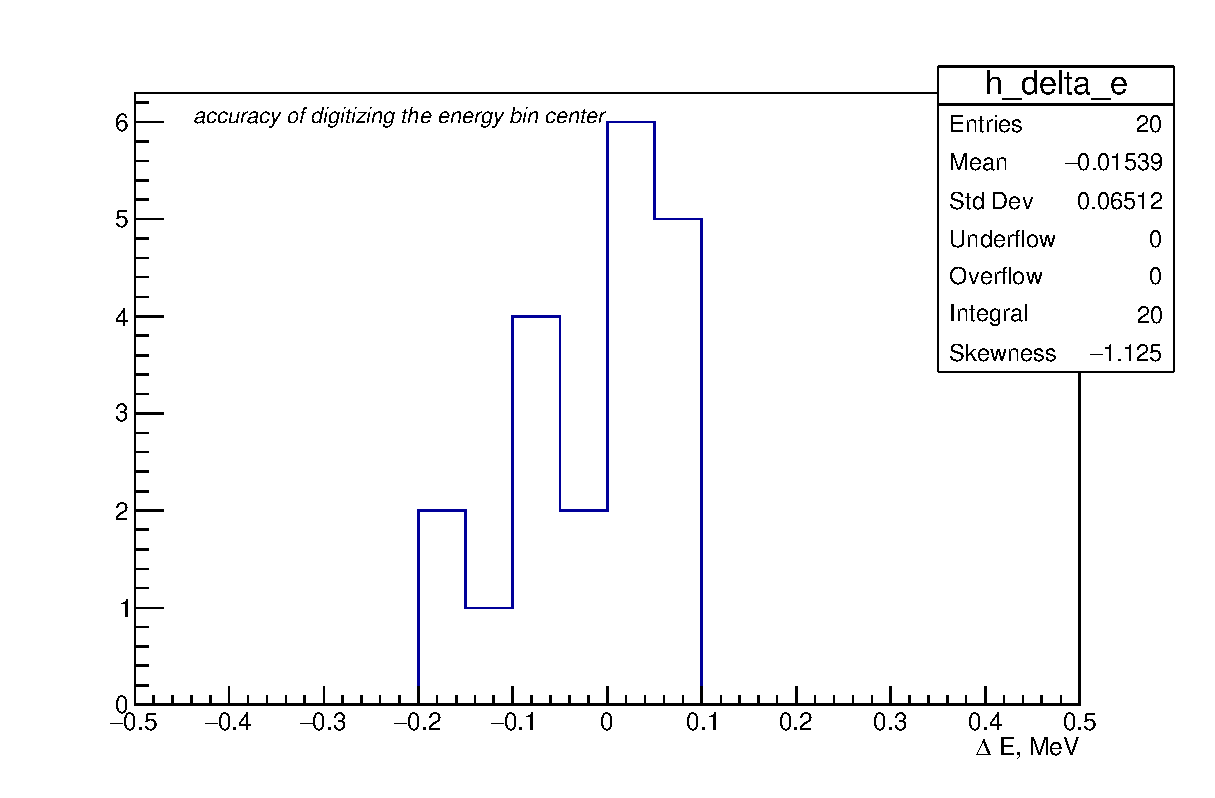
\includegraphics[width=0.49\columnwidth]{png/digitization_accuracy_de}}
    \subfloat[\label{fig:digitization_accuracy_x_y_right}]{ %
    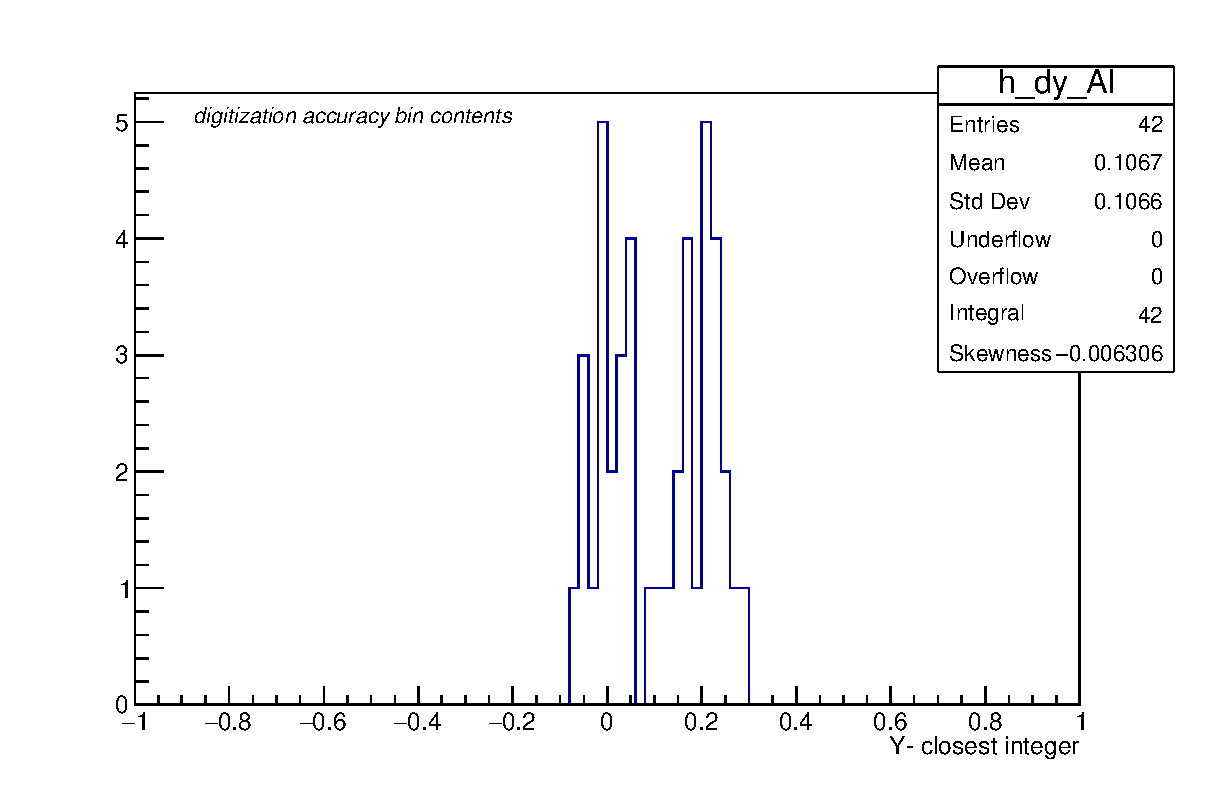
\includegraphics[width=0.49\columnwidth]{png/digitization_accuracy_Al_1992_dy} }
  \end{center}
  \caption{
    (a): accuracy of digitizing the histogram bin centers
    (b): digitization accuracy of the bin content
  }
  \label{fig:digitization_accuracy_x_y}
\end{figure}

The distribution in figure \ref{fig:digitization_accuracy_error_bars} plots the residuals
$\Delta_Y = 0.5((Y+\sigma_Y) + (Y-\sigma_Y)) - \sqrt{Y}$ for one of the digitized plots.
It confirms the assumption that the error bars on the plots are purely statistical.

\begin{figure}[htbp]
  \begin{center}
    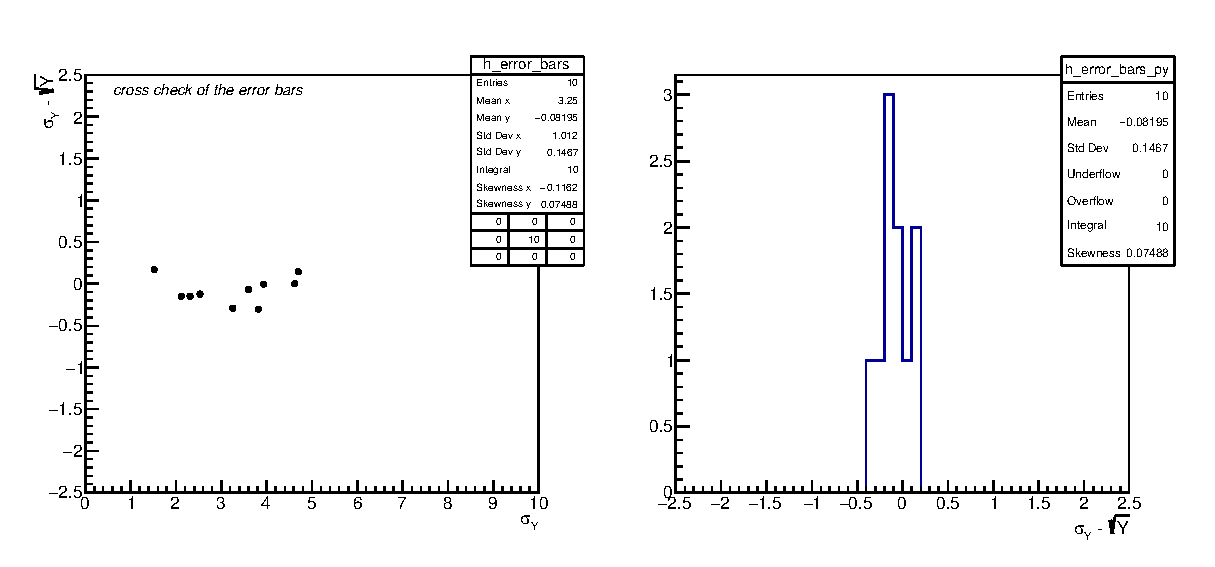
\includegraphics[width=0.99\columnwidth]{png/digitization_error_bars} 
  \end{center}
  \caption{
    left: error bar residuals, $\Delta_Y$, vs the digitized error bars
    right: y-projection of the left histogram
  }
  \label{fig:digitization_accuracy_error_bars}
\end{figure}


\section { Systematic uncertainty on the energy scale}

The energy scale of the TRIUMF RMC spectrometer has been calibrated using the
radiative pion capture (RPC) on hydrogen \cite{RMC_1992_WRIGHT_1992_249}.
Figure \ref{fig:1992_photon_spectrum_calibration} shows the measured RPC spectrum
overlayed with the simulation results. The histogram bin width
is 500 keV, and one can see that the systematic uncertainty in the reconstructed
photon energy does not exceed one bin, i.e. 0.5 MeV. Differences near 80 MeV
more likely reflect a systematics in the acceptance calculation.

\begin{figure}[htbp]
  \begin{center}
    \includegraphics[width=0.7\columnwidth]{png/1992_TRIUMF_RMC_facility_fig_9_photon_spectrum_calibration} 
  \end{center}
  \caption{
    RPC spectrum on hydrogen measured at the TRIUMF RMC spectrometer \cite{RMC_1992_WRIGHT_1992_249}.
    In the region of the RPC peak, the systematic uncertainty in the reconstructed photon energy does
    not exceed one bin, i.e. 500 keV.
  }
  \label{fig:1992_photon_spectrum_calibration}
\end{figure}

%%% Local Variables:
%%% mode: latex
%%% TeX-master: "."
%%% End:
